\section{Integrals}
\label{sec:integrals}
% From Section 3.1
\subsection{Definition of the Definite Integral}
Because the area under the curve is so important, it has a special vocabulary and notation.

\begin{definition}[The Definite Integral]
The {\bf definite integral}\index{Integral!definite}\index{Definite integral} of a positive function $f(x)$ over an interval $[a,b]$ is the area between $y=f(x)$, the $x$-axis, $x=a$, and $x=b$.

The definite integral of a positive function $f(x)$ from $a$ to $b$ is the area under the curve between $a$ and $b$.

If $f(t)$ represents a positive rate (in $y$-units per $t$-units), then the definite integral of $f(t)$ from $a$ to $b$ is the total $y$-units that {\bf accumulate}\index{Accumulation} between $t=a$ and $t=b$.

{\bf Notation for the Definite Integral.} The definite integral of $f(x)$ from $a$ to $b$ is written
$$\int_a^b f(x)\,dx \enspace .$$
The $\int$ symbol is called the {\bf integral sign}; it is an elongated letter S, standing for sum. (The $\int$ corresponds to the $\Sigma$ from the Riemann sum).

The $dx$ on the end must be included! The $dx$ tells what the variable is – in this example, the variable is $x$. (The $dx$ corresponds to the $\Delta x$ from the Riemann sum).

The function $f$ is called the {\bf integrand}\index{integrand}.

The $a$ and $b$ are called the {\bf limits of integration}\index{Limits of integration}.

{\bf Verb forms.} We {\bf integrate}, or find the definite integral of a function. This process is called {\bf integration}\index{Integration}.

\paragraph{Formal Algebraic Definition}
$$\int_a^b f(x)\,dx = \lim_{n\to\infty} \sum_{i=1}^n f(x_i)\Delta x \enspace .$$
\paragraph{Practical Definition}
The definite integral can be approximated with a Riemann sum (dividing the area into rectangles where the height of each rectangle comes from the function, computing the area of each rectangle, and adding them up). The more rectangles we use, the narrower the rectangles are, the better our approximation will be.

\paragraph{Looking Ahead}
We will have methods for computing exact values of some definite integrals from formulas soon. In many cases, including when the function is given to you as a table or graph, you will still need to approximate the definite integral with rectangles.
\end{definition}
\begin{example}
Figure \ref{fig:5-3-calls} shows $y=r(t)$, the number of telephone calls made per hour on a Tuesday. Approximately how many calls were made between 9 pm and 11 pm? Express this as a definite integral and approximate with a Riemann sum.

\begin{figure}[!ht]
  \centering
    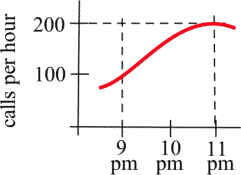
\includegraphics[width=0.3\textwidth]{img/chap5/image010.png}
    \caption{Calls per hour between 9 pm and 11 pm.}
    \label{fig:5-3-calls}
\end{figure}

\begin{solution}
We know that the accumulated calls will be the area under this rate graph over that two-hour period, the definite integral of this rate from $t=9$ to $t=11$.

The total number of calls will be $\displaystyle\int_9^{11}r(t)\,dt$.

The top of the area in Figure \ref{fig:5-3-callsapprox} is a curve, so we can’t get an exact answer. But we can approximate the area using rectangles. Let's choose to use four rectangles and left-endpoints.

\begin{figure}[!ht]
  \centering
    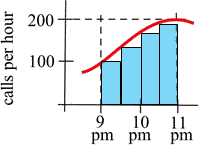
\includegraphics[width=0.4\textwidth]{img/chap5/image066.png}
    \caption{Approximating the number of calls between 9 pm and 11 pm.}
    \label{fig:5-3-callsapprox}
\end{figure}
$$\int_9^{11}r(t)\,dt\approx   0.5(100+150+180+195)=312.5 \enspace .$$
The units are (calls per hour)$\times$hours $=$ calls. Our estimate is that about 312 calls were made between 9 pm and 11 pm. Is this an under-estimate or an over-estimate?
\end{solution}\end{example}

\begin{example}
Describe the area between the graph of $f(x)=\dfrac{1}{x}$, the $x$-axis, and the vertical lines at $x=1$ and $x=5$ as a definite integral.

\begin{solution}
This is the same area we estimated to be about 1.68 before. Now we can use the notation of the definite integral to describe it. Our estimate of $\displaystyle\int_1^5\frac{1}{x}\,dx$ was 1.68. The true value of $\displaystyle\int_1^5\frac{1}{x}\,dx$ is about 1.61.
\end{solution}\end{example}

\begin{example}
Using the idea of area, determine the value of $\displaystyle\int_1^3(1+x)\,dx$.

\begin{solution}
  $\displaystyle\int_1^3(1+x)\,dx$ represents the area between the graph of $f(x)=1+x$, the $x$-axis, and the vertical lines at 1 and 3.

  \begin{figure}[!ht]
    \centering
      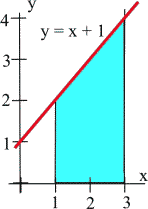
\includegraphics[width=0.3\textwidth]{img/chap5/image011.png}
      \caption{Calls per hour between 9 pm and 11 pm.}
      \label{fig:5-3-1plusx}
  \end{figure}
Since this area can be broken into a rectangle and a triangle, we can find the area exactly. The area equals
$4+\dfrac{1}{2}(2)(2)=6$.
\end{solution}\end{example}

\begin{example}
Table \ref{tab:5-3-population} shows rates of population growth for Berrytown for several years. Use this table to estimate the total population growth from 1970 to 2000:
\begin{table}[ht!]
  \centering
\begin{tabular}{lllll}
  \toprule
Year, $t$ &	1970 &	1980 &	1990 &	2000 \\
\midrule
Rate of population growth $R(t)$ in thousands of people per year &	1.5 &	1.9 &	2.2 &	2.4\\
\bottomrule
\end{tabular}
\caption{Population growth of Berrytown from 1970 to 2000.}
\label{tab:5-3-population}
\end{table}

\begin{solution}
The definite integral of this rate will give the total change in population over the thirty-year period. We only have a few pieces of information, so we can only estimate. Even though we haven't made a graph, we're still approximating the area under the rate curve, using rectangles. How wide are the rectangles? We have information every 10 years, so the rectangles have a width of 10 years. How many rectangles? Be careful here – this is a thirty-year span, so there are three rectangles.
  \begin{itemize}
    \item Using left-hand endpoints: $(1.5)(10) + (1.9)(10) + (2.2)(10) = 56$.
    \item Using right-hand endpoints: $(1.9)(10) + (2.2)(10) + (2.4)(10) = 65$.
  \end{itemize}
Taking the average of these two:
$$\dfrac{56+65}{2} = 60.5 \enspace .$$
Our best estimate of the total population growth from 1970 to 2000 is 60.5 thousand people.
\end{solution}\end{example}

\subsection{Signed Area}
You may have noticed that until this point, we've insisted that the integrand (the function we're integrating) be positive. That’s because we've been talking about area, which is always positive.

If the height (from the function) is a negative number, then multiplying it by the width doesn't give us actual area, it gives us the area with a negative sign.

But it turns out to be useful to think about the possibility of negative area. We’ll expand our idea of a definite integral now to include integrands that might not always be positive. The heights of the rectangles, the values from the function, now might not always be positive.

\begin{definition}[The Definite Integral and Signed Area]
The {\bf definite integral}\index{Definite integral}\index{Integral!definite} of a function $f(x)$ over an interval $[a,b]$ is the {\bf signed area}\index{Signed area}\index{Area!signed} between the curve $y=f(x)$, the $x$-axis, $x=a$ and $x=b$.

The {\bf definite integral} of a function $f(x)$ from $a$ to $b$ is the {\bf signed area} under the curve between $a$ and $b$.
\end{definition}
If the function is positive, the signed area is positive, as before (and we can call it area.)

If the function dips below the $x$-axis, the areas of the regions below the $x$-axis here will be negative. In this case, we cannot call it simply ``area.'' These negative areas take away from the definite integral.

$$\int_a^bf(x)\,dx = (\text{Area above } x\text{-axis}) - (\text{Area below }x\text{-axis})$$

If $f(t)$ represents a positive rate (in $y$-units per $t$-units), then the definite integral of $f(t)$ from $a$ to $b$ is the total $y$-units that accumulate between $t=a$ and $t=b$.

If $f(t)$ represents any rate (in $y$-units per $t$-units), then the definite integral of $f(t)$ from $a$ to $b$ is the net $y$-units that accumulate between $t=a$ and $t=b$.

\begin{example}
Find the definite integral of $f(x)=-2$ over the interval $[1,4]$.

\begin{figure}[!ht]
  \centering
    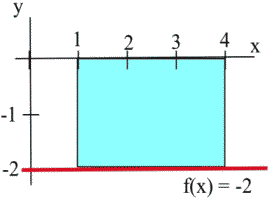
\includegraphics[width=0.3\textwidth]{img/chap5/image012.png}
    \caption{A region with negative signed area.}
    \label{fig:5-3-negative}
\end{figure}

\begin{solution}
$\displaystyle\int_1^4 -2\,dx$ is the signed area of the region shown in Figure \ref{fig:5-3-negative}. The region lies below the $x$-axis, so the area, 6, comes in with a negative sign. So the definite integral is $\displaystyle\int_1^4-2\,dx = -6$.
\end{solution}\end{example}

Negative rates indicate that the amount is decreasing. For example, if $f(t)$ is the velocity\index{Velocity} of a car in the positive direction along a straight line at time $t$ (miles/hour), then negative values of $f$ indicate that the car is traveling in the negative direction, backwards. The definite integral of $f$ is the net change in position of the car during the time interval. If the velocity is positive, positive distance accumulates. If the velocity is negative, distance in the negative direction accumulates.

This is true of any rate. For example, if $f(t)$ is the rate of population change (in people/year) for a town, then negative values of $f$ would indicate that the population of the town was getting smaller, and the definite integral (now a negative number) would be the change in the population, a decrease, during the time interval.

\begin{example}
In 1980 there were 12,000 ducks nesting around a lake, and the rate of population change (in ducks per year) is shown in Figure \ref{fig:5-3-ducks}. Write a definite integral to represent the total change in the duck population from 1980 to 1990, and estimate the population in 1990.

\begin{figure}[!ht]
  \centering
    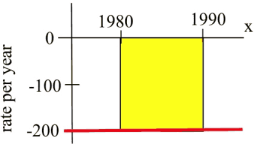
\includegraphics[width=0.3\textwidth]{img/chap5/image013.png}
    \caption{Rate of change in duck population from 1980 to 1990.}
    \label{fig:5-3-ducks}
\end{figure}

\begin{solution}
The change in population is:
\begin{align*}
  \int_{1980}^{1990}f(t)\,dt &= -(\text{area between }f\text{ and axis}) \\
    &\approx   -(200 \text{ducks/year})\cdot(10\text{ years})\\
    &= -2000\text{ ducks.}
  \end{align*}
Then (1990 duck population) $=$ (1980 population) $+$ (change from 1980 to 1990) $= (12000) + (-2000) = 10000$ ducks.
\end{solution}\end{example}

\begin{example}
A bug starts at the location $x=12$ on the $x$-axis at 1 pm walks along the axis with the velocity $v(x)$ shown in the graph in Figure \ref{fig:5-3-bug}. How far does the bug travel between 1 pm and 3 pm, and where is the bug at 3 pm?

\begin{figure}[!ht]
  \centering
    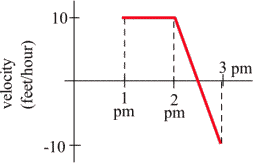
\includegraphics[width=0.3\textwidth]{img/chap5/image014.png}
    \caption{Velocity of a bug from 1 pm to 3 pm.}
    \label{fig:5-3-bug}
\end{figure}

\begin{solution}
Note that the velocity is positive from 1 until 2:30, then becomes negative. So the bug moves in the positive direction from 1 until 2:30, then turns around and moves back toward where it started. The area under the velocity curve from 1 to 2:30 shows the total distance traveled by the bug in the positive direction; the bug moved 12.5 feet in the positive direction. The area between the velocity curve and the $x$-axis, between 2:30 and 3, shows the total distance traveled by the bug in the negative direction, back toward home; the bug traveled 2.5 feet in the negative direction. The definite integral of the velocity curve, $\displaystyle\int_1^3v(t)\,dt$, shows the net change in distance:
$$\int_1^3v(t)\,dt = 12.5-2.5 = 10 \enspace .$$
The bug ended up 10 feet farther in the positive direction than he started. At 3 pm, the bug is at $x=22$.
\end{solution}\end{example}

\begin{example}
\label{ex:5-3-areas}
Use the graph in Figure \ref{fig:5-3-areas} to calculate $\displaystyle\int_0^2f(x)\,dx$, $\displaystyle\int_2^4f(x)\,dx$, $\displaystyle\int_4^5f(x)\,dx$, and $\displaystyle\int_0^5f(x)\,dx$.

\begin{figure}[!ht]
  \centering
    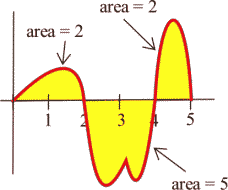
\includegraphics[width=0.3\textwidth]{img/chap5/image015.png}
    \caption{Graph for Example \ref{ex:5-3-areas}.}
    \label{fig:5-3-areas}
\end{figure}

\begin{solution}
Using the given areas, $\int_0^2f(x)\,dx = 2$, $\int_2^4f(x)\,dx = -5$, $\int_4^5f(x)\,dx = 2$, and $\int_0^5f(x)\,dx  = (\text{area above})-(\text{area below}) = (2+2)-(5)=-1$.
\end{solution}\end{example}
